\documentclass[hyperref={unicode=true}]{beamer}
\usepackage{multirow}
\usepackage{minted}
\usepackage{amsmath} % used for boldsymbol.
\renewcommand{\vec}[1]{\boldsymbol{#1}} % Uncomment for BOLD vectors.
\usepackage[slantfont,boldfont]{xeCJK}
\setCJKmainfont{SimSun}
\setCJKmonofont{FZFangSong-Z02}
\setCJKsansfont{SimHei}
\usetheme{Darmstadt}
\usecolortheme{beaver}
\usepackage{booktabs}
\usepackage{tikz}
\setbeamertemplate{theorems}[numbered]
\newtheorem{mytht}{\bf 定理}
\theoremstyle{definition}
\newtheorem{mydef}[]{\bf 定义}
\theoremstyle{proof}
\newtheorem{myprf}[]{\bf 证明}

\input zhwinfonts
\begin{document}
\setbeamertemplate{caption}[numbered]
\renewcommand\figurename{图}
\renewcommand\tablename{表}
\renewcommand\contentsname{\centering 目录}


%%------------------------------------------
\title{动态规划进阶(二)}
\subtitle{数位统计动态规划与状态压缩动态规划}
\author{马玉坤}
\institute{哈尔滨工业大学计算机科学与技术学院}
\date{2017年8月18日}
%%------------------------------------------

\begin{frame}\titlepage\end{frame}

\section{数位统计动态规划}

\subsection{理论的东西}
\begin{frame}\frametitle{数位统计动态规划}
  \begin{block}{一般形式}
    给定一个区间$[L,R]$,求在此区间内满足某个条件限制(特性)的数的个数或者加和。一般有多组询问。
  \end{block}
  \begin{exampleblock}{一般套路}
    \begin{enumerate}[<+->]
    \item 先将问题$[L,R]$转化为$[1,L-1]$和$[1,R]$的问题
    \item dp状态有两部分:
      \begin{enumerate}
      \item 跟枚举有关的部分:已枚举到的位数,以及前若干位数是不是已经到了上限(范围的限制)
      \item 跟特性有关的部分:已枚举的位上的数已经到达的状态(特性的限制)
      \end{enumerate}
    \end{enumerate}
  \end{exampleblock}
\end{frame}
\begin{frame}\frametitle{数位统计动态规划 (Cont'd)}
  \begin{alertblock}{对解题的忠告}
    \begin{enumerate}[<+->]
    \item 数位DP较容易对拍,可以本地测试,减少WA
    \item 耐心,细心
    \item 重构/重写
    \end{enumerate}
  \end{alertblock}
\end{frame}

\subsection{Find a car}
\begin{frame}{Find a car}\framesubtitle{Codeforces Round \#415 (Div. 1) C}
  \begin{block}{题目}
    给定一个无穷大的矩阵,其中第i行第j列的元素$mat(i,j)$为最小的不在集合$\{mat(1,j),mat(2,j),\ldots,mat(i-1,j), mat(i,1), mat(i,2), \ldots,mat(i,j-1)\}$中出现过的正整数。
    \begin{minipage}{0.45\linewidth}
      \begin{figure}
        \centering
        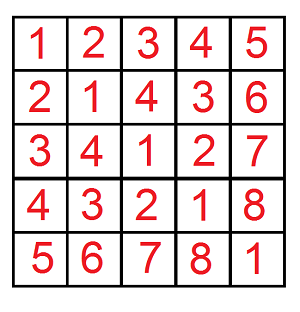
\includegraphics[width=1.2in]{figures/upper5.png}
        \caption{矩阵左上角的5个元素}\label{fig:upper5}
      \end{figure}
    \end{minipage}
    \begin{minipage}{0.45\linewidth}
      然后会有$Q(\leq 10^4)$个询问,每个询问给定$x_1,y_1,x_2,y_2,k$,回答子矩阵$(x_1,y_1)-(x_2,y_2)$内所有小于小于等于$k$的数的和。$x_1,y_1,x_2,y_2\leq 10^9$且$k\leq2\times 10^9$。
    \end{minipage}
  \end{block}
\end{frame}

\begin{frame}{Find a car (Cont'd)}\framesubtitle{Codeforces Round \#415 (Div. 1) C}
  \begin{alertblock}{第一个问题}
    第i行第j列,即$mat(i,j)$该怎么求?能不能用一个简单的式子来表示?\\
    \pause{}先把矩阵里的每个元素都减1,行数和列数从1开始变为从0开始。\\
    \pause{}此时可转化为两堆石子(分别为$i$和$j$),做NIM游戏。$mat(i,j)=\text{各个子状态的SG函数}=i \oplus j$ ($\oplus$为异或)。对于原矩阵就有$mat(i,j)=(i-1)\oplus (j-1) + 1$。\\
    {\bf 不懂原理也没关系,今天我们的重点不在这。}
  \end{alertblock}
\end{frame}

\begin{frame}{Find a car (Cont'd)}\framesubtitle{Codeforces Round \#415 (Div. 1) C}
  \begin{block}{异或}
    \begin{figure}
      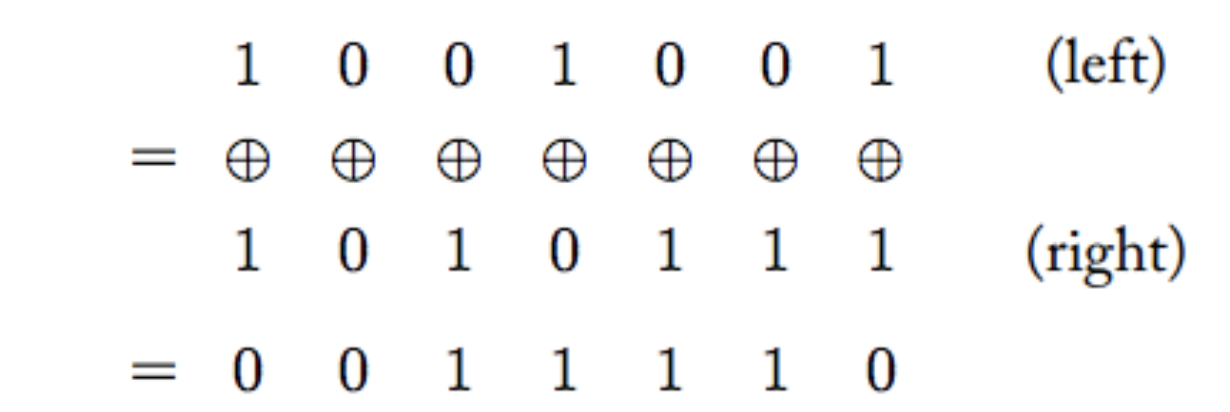
\includegraphics[width=2.3in]{figures/xor.png}
      \caption{异或}\label{fig:xor}
    \end{figure}
  \end{block}
\end{frame}

\begin{frame}{Find a car (Cont'd)}\framesubtitle{Codeforces Round \#415 (Div. 1) C}
  \begin{block}{二维前缀和}
    设$sum(x,y)=\sum_{i=1}^x \sum_{j=1}^j a(i,j)$,那么我们有
    \begin{align}
      &\sum_{i=x_1}^{x_2} \sum_{j=y_1}^{y_2} a(i,j)\\
      =&sum(x_2,y_2)-sum(x_1-1,y_2)\\
      &-sum(x_2,y_1-1)+sum(x_1-1,y_1-1)
      \end{align}
  \end{block}
\end{frame}

\begin{frame}{Find a car (Cont'd)}\framesubtitle{Codeforces Round \#415 (Div. 1) C}
  \begin{exampleblock}{数位DP}
    问题转化成求$\sum_{i=1}^{x}\sum_{j=1}^{y}[i\oplus j\leq k](i \oplus j)$\\
    设$f(di,dx,dy,dk)$为这个状态下的数字个数,$g(di,dx,dy,dk)$为数字和。其中$di$表示从最高位开始已枚举到的位数,$dx,dy$分别表示已枚举的$x$与$y$的前缀是否到达上限,$dk$表示已枚举的$x$和$y$的前缀的异或是否达到$k$的上限。\\
    详见代码。
  \end{exampleblock}
\end{frame}

\begin{frame}{Find a car (Cont'd)}\framesubtitle{Codeforces Round \#415 (Div. 1) C}
  \begin{exampleblock}{数位DP (Cont'd)}
    为什么这样设计状态?举个例子。\\
    比如$x=1010,y=0101,k=1110$,枚举完了高三位,此时已枚举的$x'=101$,$y'=010$,且它们的异或值$k'=111$,这时候的状态应该是$f(0,1,1,1)$(枚举到第0位,且$x,y,k$前缀都达到限制)。\\
    那么我们枚举低位的时候就不能随便枚举$x$和$y$,否则会超出$x$和$y$的限制。同时,我们还要注意已枚举的前缀是否达到$k$的上限,如果达到了$k$的上限,同样不能随便枚举$x$和$y$。枚举第0位时,我们实际上x只能取0,y只能取0或1,但y不能取1,因为这时候$x\oplus y=1111$,超出了范围。
  \end{exampleblock}
\end{frame}

\begin{frame}{Find a car (Cont'd)}\framesubtitle{Codeforces Round \#415 (Div. 1) C}
  \begin{exampleblock}{总结}
    四个状态中前三个状态(位数,x前缀,y前缀)都是关于枚举的范围的,而第四个状态可以理解成枚举的范围,也可以理解成数的特性。在这里我们使用了布尔变量,表示前缀是否达到上限,从而使得我们枚举后面的位时知道是否需要注意范围的限制。
  \end{exampleblock}
\end{frame}

\subsection{两种dp数组求解的写法}
\begin{frame}[fragile]{递推求动态规划}
  \begin{minted}{C++}
for (int i = 0; i < n; i++) {
  for (int j = volume[i]; j <= capacity; j++) {
    dp[i][j] = max(dp[i-1][j], dp[i-1][j-volume[i]] + value[i]);
  }
}
  \end{minted}
\end{frame}

\begin{frame}[fragile]{递归求动态规划(记忆化搜索)}
  \begin{minted}{C++}
int dfs(int i, int j) {
  if (i == 0) {
    return 0;
  }
  if (vis[i][j]) {
    return dp[i][j];
  }
  vis[i][j] = 1;
  return dp[i][j] = max(dfs(i-1, j-1),
                        dfs(i-1, j-volume[i]) + value[i]);
}
  \end{minted}
\end{frame}
\begin{frame}{两种方法的比较}
  \begin{itemize}[<+->]
  \item 递推的优势
    \begin{enumerate}
    \item 常数小
    \item 不需递归,不怕爆栈
    \end{enumerate}
  \item 递归的优势
    \begin{enumerate}
    \item 对有效状态数较少的问题可大大提高效率,避免无效状态的搜索
    \item 实现简单,更符合人类思维
    \end{enumerate}
  \end{itemize}
\end{frame}


\subsection{K-wolf Number}
\begin{frame}{K-wolf Number (Cont'd)}\framesubtitle{2016 Multi-University Training Contest 5 07}
  \begin{block}{问题}
    K-wolf数字定义为:十进制表示下,任意相邻的k位数字都各不相同。\\
    给定$L,R,K$,求区间$[L,R]$内的K-wolf数字的个数。\\
    $L,R\leq10^{18};K\leq5$
  \end{block}
\end{frame}

\begin{frame}{K-wolf Number (Cont'd)}\framesubtitle{2016 Multi-University Training Contest 5 07}
  \begin{exampleblock}{解法}
    转化为$1,\ldots,n$的K-wolf数个数的问题。\\
    设$dp(i,j,k)$表示从最高位枚举到第i位,j表示已枚举的位有没有达到n的上限,k存的是已枚举的位中后k-1位的值。这样我们就能知道。\\
  \end{exampleblock}
\end{frame}

\begin{frame}{K-wolf Number (Cont'd)}\framesubtitle{2016 Multi-University Training Contest 5 07}
  \begin{exampleblock}{解法 (Cont'd)}
    注意到一个问题:刚才的题目 (Find a car)中,我们实际上将所有数都加上了前导零,补成了31位。然而在这个题目中,如果我们仍然这么操作,从第8位开始枚举,补上前导零,把所有数都变成18位数,那么像29这样的数就会变成000000000000000029,不符合K-wolf数的定义 (有连续的0),所以我们不能算上前导零。\\
    \pause{}一种方案是:在dp状态中,加入一维指示之前枚举的位是否全是0。\\
    另一种方案是:手动枚举数的位数以及最高位的数字,然后剩下再dp。
  \end{exampleblock}
\end{frame}

\begin{frame}{K-wolf Number (Cont'd)}\framesubtitle{2016 Multi-University Training Contest 5 07}
\end{frame}

\section{状态压缩动态规划}

\begin{frame}{Stabilization}\framesubtitle{2016 Multi-University Training Contest 6 06}
\end{frame}

\end{document}
